% including these three lines add line numbers to the draft.
%\RequirePackage{lineno} \setlength{\linenumbersep}{6pt} \linenumbers

\documentclass[11pt]{article}

% To use the \includegraphics package we usually use:
\usepackage{graphicx} %dblfloatfix}   % Include figure files
\usepackage{subfigure}
\usepackage{array}
\usepackage{amsmath}
\usepackage{multirow}
\usepackage{cite}
\usepackage{url}
\usepackage{authblk}
\usepackage[margin=1.5cm]{geometry}
\usepackage{amssymb}																
\usepackage{pstricks,pst-grad}							
\usepackage{subfigure}								
%\usepackage{lineno}							      
%\linenumbers		


\textheight = 43\baselineskip
\advance\textheight by \topskip

%
% $Id: abrev.tex,v 1.7 2006/05/26 18:24:40 gsfs Exp $
%

\newcommand{\bs  }{$\backslash\!$     }
%
%
%%%%%%%%%%%%%%%%%%%%%%%%%%%%%%%%%%%%%% definitions initiales
\newcommand{\arw}{ $\rightarrow$ }
\newcommand{\dg}{$^\circ$}
\newcommand{\x}{$\times$}
\newcommand{\tbox}[1]{\mbox{#1}}
\newcommand{\LUMI}{$\mathcal{L}$}
\newcommand{\lumi}[1]{$10^{#1} {\rm ~cm}^{-2}{\rm s}^{-1}$}
\newcommand{\Lumi}[1]{$\mathcal{L}=10^{#1} {\rm ~cm}^{-2}{\rm s}^{-1}$}
\newcommand{\sd}{\bfseries\itshape\large}
\newcommand\ie {{\it i.e.}}
\newcommand\eg {{\it e.g.}}
\newcommand\etc{{\it etc.}}
\newcommand\cf {{\it cf.}}
\newcommand\etal {{\it et al.}}
\newcommand{\be}{\begin{eqnarray}}
\newcommand{\ee}{\end{eqnarray}}
%\def\mupmum{\mu^+\mu^-}
\def\mz{m_Z}
\def\gev{\,{\rm GeV}}
\def\tev{\,{\rm TeV}}
\def\rts{{\sqrt s}}
\def\gam{\gamma}
\def\G{\gamma}
\def\GG{\gamma\gamma}
\def\EPEM{e^+e^-}
\def\MUPM{\mu^+\mu^-}
\def\A{\alpha}
\def\ZA{Z\alpha}
\def\BE{\begin{equation}}
\def\EE{\end{equation}}
\def\fbi{~{\rm fb}^{-1}}
\def\lsim{\mathrel{\raise.3ex\hbox{$<$\kern-.75em\lower1ex\hbox{$\sim$}}}}
\def\gsim{\mathrel{\raise.3ex\hbox{$>$\kern-.75em\lower1ex\hbox{$\sim$}}}}
\def\to{\rightarrow}
\def\la{\mathrel{\mathpalette\fun <}}
\def\ga{\mathrel{\mathpalette\fun >}}
\def\fun#1#2{\lower3.6pt\vbox{\baselineskip0pt\lineskip.9pt}}
%%%%%%%%%%%%%%%%%%%%%%%%%%%%%%%%%%%%%%%%%%%%%%%%%%%%%%%%%%%%%%%%%%
\makeatletter
\def\lesssim{\mathrel{\mathpalette\vereq<}}
\def\vereq#1#2{\lower3pt\vbox{\baselineskip1.5pt \lineskip1.5pt
\ialign{$\m@th#1\hfill##\hfil$\crcr#2\crcr\sim\crcr}}}
\def\gtrsim{\mathrel{\mathpalette\vereq>}}
\makeatother
%%%%%%%%%%%%%%%%%%%%%%%%%%%%%%%%%%%%%%%%%%%%%%%%%%%%%%%%%%%%%%%%%%
%
% Celles que j'ai definies ou re-utilisees
%
%\newcommand{\sigtot}{$\sigma^{\mathrm {tot}$}     % sigma_tot
\def\sigtot{$\sigma^{\mathrm {tot}}$}     % sigma_tot
%\newcommand{\sigabs}{$\sigma_{\mathrm {abs}}$}     % sigma_abs
\def\sigabs{$\sigma^{\mathrm {abs}}$}
\newcommand{\sigel}{$\sigma^{\mathrm {el}}$}     % sigma_el
\newcommand{\siginel}{$\sigma^{\mathrm {inel}}$}     % sigma_in
%
\newcommand{\lgl}{$\langle$}
\newcommand{\rgl}{$\rangle$}
%
\newcommand{\gamgam  }{$\gamma\gamma$}
%\newcommand{\gam     }{$\gamma$ }
\newcommand{\positon }{$e^+$}
\newcommand{\electron}{$e^-$}
\newcommand{\epem    }{$e^+e^-$}
%
\newcommand{\muon    }{$\mu$}
\newcommand{\mumu    }{$\mu\mu$}
\newcommand{\mup     }{$\mu^+$}
\newcommand{\mum     }{$\mu^-$}
\newcommand{\mupm    }{$\mu^{\pm}$}
\newcommand{\mmpm    }{$\mu^+\mu^-$}
\def\mupmum{\mu^+\mu^-}
\newcommand{\mupmup  }{$\mu^+\mu^+$}
\newcommand{\mummum  }{$\mu^-\mu^-$}
\newcommand{\muo     }{$\mu^0$\ }
%
\newcommand{\w}{$W$\ }
%
\newcommand{\kaon  }{$K$}
\newcommand{\ko    }{$K^0$}
\newcommand{\kp    }{$K^+$}
\newcommand{\km    }{$K^-$}
\newcommand{\kpm   }{$K^{\pm}$}
\newcommand{\pip   }{$\pi^+$}
\newcommand{\pim   }{$\pi^-$}
\newcommand{\pio   }{$\pi^0$}
\newcommand{\pipm  }{$\pi^{\pm}$}
%
\newcommand{\jpsi}{$J/\psi$}
\newcommand{\psip}{$\psi^{\prime}$}
%
\newcommand{\ups}{$\Upsilon$}
\newcommand{\upsp}{$\Upsilon^{\prime}$}
\newcommand{\upspp}{$\Upsilon^{\prime\prime}$}
%
\newcommand{\wpm  }{$W^{\pm}$}
\newcommand{\zo   }{$Z^0$}
%
\newcommand{\ro    }{$\rho$}
\newcommand{\omga  }{$\omega$}
\newcommand{\ffi   }{${\it\Phi}$}
\newcommand{\qqb   }{$q\overline q$}
\newcommand{\ccb   }{$c\overline c$}
\newcommand{\bbb   }{$b\overline b$}
\newcommand{\ppb   }{$p\overline p$}
%
%                                                 systemes
\newcommand{\pp}{p+p}           % pp
\newcommand{\eecol}{e$^+$+e$^-$}           % pp
\newcommand{\eA}{e+A}           % pp

\newcommand{\pn}{p+n}           % pn
\newcommand{\pd}{p+d}           % pd
\newcommand{\pA}{p+A}           % pA
\newcommand{\pca}{p+Ca}           % pA
\newcommand{\pPb}{p+Pb}           % pPb
\newcommand{\aacol}{A+A}                 % AA
\newcommand{\pbpb}{Pb+Pb}           % PbPb
\newcommand{\PbPb}{Pb+Pb}           % Pb+Pb
\newcommand{\AuAu}{Au+Au}           % Au+Au
\newcommand{\SnSn}{Sn+Sn}           % Sn+Sn
\newcommand{\KrKr}{Kr+Kr}           % Kr+Kr
\newcommand{\ArAr}{Ar+Ar}           % Ar+Ar
\newcommand{\NbNb}{Nb+Nb}           % Nb+Nb
\newcommand{\OO}{O+O}           % O + O
%
%                                                 baryons
\newcommand{\p}{$p$}                              %
\newcommand{\n}{$n$}                              %
%
%
%
%  dans les textes                                                 variables
\newcommand{\ycms}{$y_{\rm c.m.s.}$}
\newcommand{\ylab}{$y_{\rm lab}$}
\newcommand{\etta}{$\eta$}
\newcommand{\abseta}{$\vert\eta\vert$}
\newcommand{\absetamu}{$\vert\eta_{\mu}\vert$}
\newcommand{\dsigdt}{d$\sigma$/d$t$}
\newcommand{\Ncol}{$N_{\rm col}$}                    %  dN/dy
\newcommand{\dnchdy}{d$N$/d$y$}                    %  dN/dy
\newcommand{\dnpmdy}{d$N^{\pm}$/d$y$}                    %  dN+-/dy
\newcommand{\dndeta}{d$N$/d$\eta$}               % dN/deta
\newcommand{\dEdy}{d$E$/d$y$}                    % dE/dy
\newcommand{\dEdx}{d$E$/d$x$}                    % dE/dx
\newcommand{\dedx}{{\rm d}E/{\rm d}x}          % dE/dx mod math
\newcommand{\dEdeta}{d$E$/d$\eta$}                % dE/deta

\newcommand{\sqrs}{$\sqrt{s}$}
\newcommand{\Et}{$E_{\rm T}$}                    % E_T
\newcommand{\pl}{$p_{\rm L}$}                    % p_T
\newcommand{\pt}{$p_{\rm T}$}                    % p_T
\newcommand{\pto}{$p_{\rm T}^0$}                    % p_T^0
\newcommand{\ptmu}{$p_{\rm T}^{\mu}$}                    % p_T
\newcommand{\po}{$p_\mathrm 0$}                    % p_0
\newcommand{\plab}{$p_\mathrm {lab}$}                % p_Lab     %
\newcommand{\ptcut}{$p_{\rm T}^{\rm cut}$}                % p T cut
\newcommand{\ptmin}{$p_{\rm T}^{\rm min}$}                % p T cut
\newcommand{\ptlin}{$p_{\rm T}^{\rm lin}$}                % p T cut
%
%                                                 decay
%                                                 decay
%                                                 unite
\newcommand{\Gevc}{GeV/$c$}                      % GeV/c
%
%                                                 coordonnees
\newcommand{\xcor}{$x$}
\newcommand{\ycor}{$y$}
\newcommand{\zcor}{$z$}
\newcommand{\rcor}{$r$}
\newcommand{\abz}{$\vert z\vert$}
\newcommand{\fiangle}{$\varphi$}
\newcommand{\tetangle}{$\theta$}
\newcommand{\deltafi}{$\Delta\varphi$}
%
\newcommand{\micron}{$\mu$m}
\newcommand{\diffd}{{\rm d}} % forme differentielle droite dans les formules math


% Insert macros here
\newcommand{\myZ}{\rm{Z}^0}
\newcommand{\myW}{\rm{W}^\pm}
\newcommand{\myJ}{J/\psi}
\newcommand{\ET}{E_T}
\newcommand{\pT}{p_T}
\newcommand{\smallurl}[1]{{\small{\url{#1}}}}
\newcommand{\dndy}{dN_{\rm ch}/d\eta}
%\newcommand{\dnchdy}{\rm{dN}_{\rm ch}/\rm{d}\eta}
\newcommand{\nch}{N_{\rm ch}}
\newcommand{\deta}{\rm{d}\eta}
\newcommand{\dNdeta}{dN_{\rm ch}/d\eta|_{\eta=0}}
\newcommand{\dpT}{dp_T}
\newcommand{\dphi}{d\phi}
\newcommand{\evtAdigihits}{300051}
\newcommand{\evtArechits}{70846}
\newcommand{\eVperElectron}{3.7}
\newcommand{\electronsPerADC}{135}
\newcommand{\keVperTwoADCs}{1}
\newcommand{\noiseThreshold}{3.7037}
\newcommand{\pixelThresholdInNoiseUnits}{5}
\newcommand{\pixelThresholdInADCcounts}{18}
\newcommand{\seedThresholdInNoiseUnits}{6}
\newcommand{\seedThresholdInADCcounts}{22}
\newcommand{\clusterThresholdInNoiseUnits}{10.1}
\newcommand{\clusterThresholdInADCcounts}{38}
\newcommand{\tracks}{\texttt{tracks()}}
\newcommand{\defaultfilter}{\texttt{SimpleCarfSimTrackFilter}}
\newcommand{\trackerboundsradius}{\texttt{TrackerBounds::\-radius()}}
\newcommand{\trackerboundshalflength}{\texttt{abs(TrackerBounds::\-halfLength())}}
\newcommand{\openfiltertksimtrack}{\texttt{OpenFilter<TkSimTrack>}}













\usepackage{fancyhdr}
\pagestyle{fancy}
\fancyhf{}
\headheight 15pt
\usepackage{lastpage}
\cfoot{\thepage\ }
\renewcommand{\footrulewidth}{0pt}
\renewcommand{\headrulewidth}{0pt}
\setlength{\topmargin}{0in}

\usepackage{paralist}
\def\titlepage{\clearpage%
\setcounter{footnote}{0}\pagestyle{empty}}

\def\@makefnmark{\hbox{$^{\@thefnmark)}$}}
\def\author#1{%% Treat the list of authors
\setcounter{footnote}{0}\def\@currentlabel{}%
\begingroup\def\thefootnote{\arabic{footnote}}
\def\@makefnmark{\hbox{$^{\rm\@thefnmark)}$}}
\global\@topnum\z@ \begin{center}{\lineskip.5em
\begin{tabular}[t]{c}#1\end{tabular}\par}
\end{center}\par\vskip1.5em\@thanks\endgroup}
\newenvironment{Authlist}{\center}{\endcenter}

\def\date#1{{\large\bf\hfill #1}}
\def\title#1{\vskip1.5cm\begin{center}\huge\sf#1\end{center}\vskip1.5em}
\providecommand{\fixme}[1]{{\sffamily{\bfseries{}FIXME:} #1}}
\providecommand{\FIXME}[1]{{\sffamily{\bfseries{}FIXME:} #1}}

%\singlespace
%\date{\today}

\pagestyle{fancy}
\setcounter{page}{1}
\pagenumbering{arabic}
\begin{document}

\begin{titlepage}
\vspace{2.2 cm}
\title{\textbf{Neutrinos reconstruction in DUNE experiment using Machine Learning}}

\vspace{.2 cm} 

\begin{center}
\begin{tabular}{ll}
 
\textbf{Principal Investigator:} & Prof. Edward Blucher \\
\textbf{Institution:}                    & University of Chicago \\
\textbf{Phone:}  		      & (+1) 773-702-7486 \\
\textbf{E-mail:}  		      & blucher@hep.uchicago.edu \\
& \\
\textbf{Principal Investigator:}  & Camelia Mironov \\
\textbf{Institution:}                    & CNRS-IN2P3, Laboratoire APC Paris\\
\textbf{Phone:} & 			 (+40) 755-345-190 \\
\textbf{E-mail:} & 			 mironov@apc.in2p3.fr \\
& \\
\end{tabular}

\vspace{2 cm} 
\textbf{This application is submitted for consideration within the\\ UChicago - CNRS Collaboration Program}

\end{center}



\end{titlepage}







\pagestyle{fancy}
\setcounter{page}{1}
\pagenumbering{arabic}

\section{Part B: Description of the Project}
\vspace{-0.3cm}
\paragraph{State of the art for the research area.} The Deep Underground Neutrino Experiment (DUNE) is a state of the art next generation neutrino-oscillation experiment, which will be installed in the Long-Baseline Neutrino Facility (LBNF), under construction now in the United States. When completed, LBNF/DUNE will be the largest experiment ever built in the US to study the properties of the long-discovered (yet still mysterious) particles called neutrinos and of their antimatter counterparts, antineutrinos. The planned studies aim to measure unknown parameters of the Standard Model of particle physics, facilitate the search for new phenomena, and overall answer fundamental questions about the evolution of the universe and the nature of its matter. The world’s most intense neutrino beam will be produced at the Fermi National Accelerator Laboratory (FNAL) in Batavia, Illinois, by smashing accelerated protons into a target. Neutrino measurements will be performed with two detectors: a `Near Detector’ (ND), installed in FNAL, will record the particle interactions near the source of the beam; and a `Far Detector’ (FD) which will be installed more than a kilometer underground and 1,300 kilometers downstream of the source, at the Sanford Underground Research Laboratory (SURF) in Lead, South Dakota. This will be the longest distance of any experiment with man-made neutrinos. The extraordinary world-wide financial, engineering, and overall scientific commitments are proof of the importance of the expected DUNE physics program. 
\vspace{-0.5cm}
\paragraph{Description of the project and domains of interest; quality and originality of the project.} The aim of the proposed project is to develop innovative algorithms to optimize the reconstruction of neutrino interactions in the DUNE Far Detector, exploiting the full potential of the detector design in order to maximize the sensitivity to neutrino oscillation parameters. 

\vspace{-0.2cm}
\begin{figure}[!ht]
\begin{center}
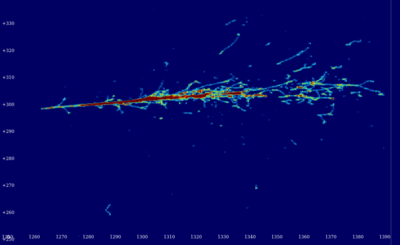
\includegraphics[width=.35\textwidth, height=4cm]{eNu_event}
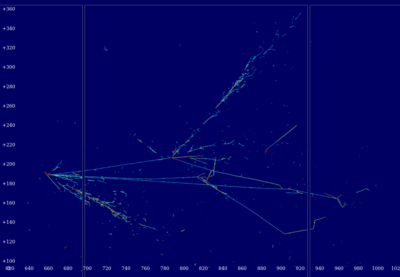
\includegraphics[width=.35\textwidth, height=4cm]{muNu_event}
\vspace{-0.5cm}
\caption{Electron- (left) and a Muon-neutrino (right) decay in LAr TPC.}
\label{fig:evDisplay}
\end{center}
\end{figure}
\vspace{-0.5cm}

Neutrinos (and their antimatter counterparts, antineutrinos) are very difficult to study, because they pass through most matter without leaving a trace. To identify them, enormous detectors are needed. The DUNE Far Detector is such an instrument. It consists of four massive Time Projection Chambers (TPC) modules, each longer than an Olympic-size swimming pool, and four stories tall. Together, they will hold 70,000 tons of liquid argon (LAr), a crystal clear material that is ideal for the detailed measurement of neutrino interactions [1]. The Far Detector is designed to search for physics beyond the Standard Model, and to observe neutrinos from a Galactic Core-Collapse SuperNova should one occur. The LAr TPCs will provide high-resolution images of neutrino events, as shown in Fig.~\Ref{fig:evDisplay}. In such frames, the challenge is to identify track versus shower particle trajectories, kinks and wiggles (which can tell the momentum of the particle that produced them), any small traces (which can inform on the direction and guide global topology reconstruction) and energy depositions (which can inform on the particle energy and type). In addition, separating known signal (from a real, known physics process), from fake signal (due to detector noise or other technical problems), from novel signal (real signal but from a  not-yet discovered physics process) is the ultimate challenge. Given the complexity of the scientific problem, a more sophisticated reconstruction approach should be developed to fully exploit the high-resolution detection technology. We plan to develop a Machine Learning (ML) based framework, to perform neutrino event reconstruction in the FD of the DUNE experiment. We will join in this approach an effort that is in its infancy in the DUNE community, but which has already attracted interest from a few other universities and laboratories in US (UC Berkeley, Lawrence Berkeley National Laboratory, MIT, SLAC, Stanford). 
\vspace{-0.5cm}
\paragraph{Objectives, methodology, expected results and their relevance.} We propose to use Convolutional Neural Networks for classification of the LAr TPC images, to distinguish electron-neutrinos from muon-neutrinos, and identify neutral-current interactions.  While this approach has already been proven to improve the sensitivity to neutrino oscillation parameters, the proposal aims to go beyond. By applying Deep Learning techniques, we plan to reconstruct the neutrino energy, with the aim of minimizing the systematic effects due to the detector and to the incomplete knowledge of neutrino interaction models. We will also explore the possibility to use Graph Neural Networks to achieve the best determination of the energy of the event, including the details of  individual particles produced in the neutrino interactions, such as neutrons or protons. The full capabilities of the Liquid Argon TPC, which will provide multi-dimensional input including timing and position reconstruction in the two views, as well as charge deposition, will be exploited. The main output will be the neutrino energy, with  additional information (such as event type tagging, direction, etc) also to be pursued. Large samples of simulated data will be used to study the performance of the implemented framework. Special focus will be devoted to the optimization of the input images and of the network architecture, in order to make the computing time acceptable for DUNE data samples, while not losing relevant information. Studies will be performed to evaluate the improvement in the resolution on the neutrino energy and the impact of the different systematic effects. Finally, the sensitivity to neutrino oscillation parameters will be assessed. 
\vspace{-0.5cm}
\paragraph{Future perspectives.} The immediate extension of a successful ML reconstruction approach for the FD, will be event reconstruction in the ND. The added complication for the ND is the occurrence of pileup events: more neutrino-events appearing simultaneously in the detector, resulting in one picture in which many frames as the ones shown in Fig.~\Ref{fig:evDisplay} are overlapped. 
\vspace{-0.5cm}
\paragraph{Supervision and mentorship of PhD students.} At APC, the candidates will be supervised by Camelia Mironov, Director of Research at CNRS, who recently joined the DUNE Collaboration bringing a strong experience on data analysis from heavy ion physics. She will be flanked by the other members of the team: Prof. Thomas Patzak (team leader), Prof. Alessandra Tonazzo (also in charge of the STEP'UP Doctoral School), Dr Jaime Dawson and Dr Sabrina Sacerdoti, who have a leading role in the development of the readout for the DUNE photon detection system. At UChicago, mentoring will be provided by Prof. Ed Blucher, former co-spokesperson of the DUNE Collaboration, who have been deeply involved in DUNE program since the start of the experiment.
\vspace{-0.5cm}
\paragraph{Enhancement of the project due to collaboration.} There are currently two TPC designs being planned for Far Detector modules: Horizontal Drift (HD) with charge readout based on wire planes, and Vertical Drift (VD) using printed circuit boards.  Both technologies are currently being prototyped at CERN, with significant contribution from CNRS and UChicago researchers in many aspects: prototypes' construction, developments of electronics and data acquisition, simulation and data analysis preparations. The PhD candidates will largely benefit from the complementary expertise of the APC and UChicago groups in terms of technical contributions to the DUNE experiment. The common interest of the two groups in the development of Machine Learning techniques for the two detector technologies (HD and VD) and their application to ProtoDUNE (DUNE FD-prototype at the CERN Neutrino Platform) data will be a unique opportunity for them to rapidly gain experience on these topics.
\vspace{-0.5cm}
\paragraph{Synergy between research theme and laboratory.}
There are currently two TPC designs being planned for Far Detector modules: Horizontal Drift (HD) with charge readout based on wire planes, and Vertical Drift (VD) using printed circuit boards.  Both technologies are currently being prototyped at CERN, with significant contribution from CNRS and UChicago researchers in many aspects: prototypes' construction, developments of electronics and data acquisition, simulation and data analysis preparations. The PhD candidates will largely benefit from the complementary expertise of the APC and UChicago groups in terms of technical contributions to the DUNE experiment. The common interest of the two groups in the development of Machine Learning techniques for the two detector technologies (HD and VD) and their application to ProtoDUNE ( DUNE Far Detector prototype at the CERN Neutrino Platform) data will be a unique opportunity for them to rapidly gain experience on these topics.



\clearpage



\section{Part C: Added value of the international cooperation}

\textit{Benefits of the international cooperation.}


\textit{Expected benefits for the French and US teams.} 

\textit{Balance between the contributions of the French and US teams.}

\textit{Role of additional industrial/governmental collaborations.}




\clearpage



\newpage

\end{document}
